\documentclass{ctexart}
\usepackage{tabularx}
\usepackage{amssymb} 
\usepackage{amsmath}
\usepackage{graphicx}
\author{JohnsonLee}
\title{多元函数微分学及其应用}
\date{\today}

\begin{document}
  \begin{titlepage}
    \maketitle
    \tableofcontents
  \end{titlepage}
  \section{多元函数的基本概念}
    \subsection{区域}
      \subsubsection{邻域}
      \paragraph{邻域}
        设$P_0(x_0,y_0)$是$xOy$平面上的一个点,$\delta$是一个正数$(\delta > 0)$,与点$P_0(x_0,y_0)$距离小于$\delta$的点$P(x,y)$的全体,称为$P_0$的$\delta$领域,记为$U(P_0,\delta)$.
        $$P_0 = \{(x,y)|(x-x_0)^2 + (y-y_0)^2 < \delta\}$$
      \paragraph{去心邻域}
        在邻域$U(P,\delta)$中除去点$P_0$得到的平面点集,成为点$P_0$的去心邻域.
        $$P_0 = \{(x,y)|0<(x-x_0)^2 + (y-y_0)^2 < \delta\}$$
    点$P$邻域和去心领域分别记作$U(P)$和$U^0(P)$
      \subsubsection{内点、外点、边界点和聚点}
        设$E$是平面上的一个点集,$P$是平面上的一个点.
        \begin{table}[htbp]
          % \caption{}
          \centering
          \begin{tabularx}{\textwidth}{|l|X|X|}
            \hline
            名称&定义&通俗解释\\ \hline
            内点&若\emph{存在}$\delta$ > 0,使得$U(P,\delta) \subset E$,则成$P$为$E$的内点&可以找到一个能完全被E框住的邻域\\ \hline
            外点&若存在$\eta > 0,$使得$U(P,\eta) \cap E = \emptyset$,则称$P$为$E$的外点&可以找到一个跟$E$不沾边的邻域\\ \hline
            边界点&若任意$\epsilon$ > 0,在$U(P,\epsilon)$内既有$E$的点又有不属于$E$的点,则称P为E的边界点 & 边界点的邻域总是一部分$E$在外面,一部分在$E$里面\\ \hline
            聚点&若任意$\epsilon$ > 0,总有$U^0(P,\epsilon) \cap E \neq \emptyset$,则称点$P$为$E$的聚点&对于点$P$的一个邻域再小都好,总是和E相交\\ \hline
            孤立点&若存在$\epsilon$ > 0,使得$U(P,\epsilon) \cap E = \{P\}$,则称点$P$为$E$的孤立点&首先$P$在$E$内,那么外点肯定不是孤立点,$P$应该是$E$的集合中一个特殊的点\\ \hline
          \end{tabularx}
        \end{table}
        \paragraph{注意:}
          \subparagraph{1.点的类型}任给一个点$P$,要么是$E$的内点,要么是外点,要么是边界点。
          \subparagraph{2.内点外点等的关系}$E$的内点属于$E$,$E$的外点不属于$E$,$E$的边界点可能属于$E$,也可能不属于$E$,$E$的边界点的全体成为E的边界,记作$\partial E$
          \subparagraph{3.}孤立点属于$E$,孤立点也是边界点.
          \subparagraph{4.}聚点可能属于$E$,也有可能不属于$E$.
          \subparagraph{5.}边界点$\subseteq$ 聚点+孤立点,不是聚点的边界点一定是孤立点,故其属于E
          \subparagraph{6.}内点是聚点.外点肯定不是聚点.
          \subparagraph{7.}聚点 $\subseteq$ 内点+边界点
        \paragraph{一个例子}
          \begin{quote}
            $$E = \{(x,y)|x^2+y^2 = 0 或 1 < x^2+y^2 \leq 4\}$$
            \begin{figure}[p]
            \centering
            \caption{例一}
            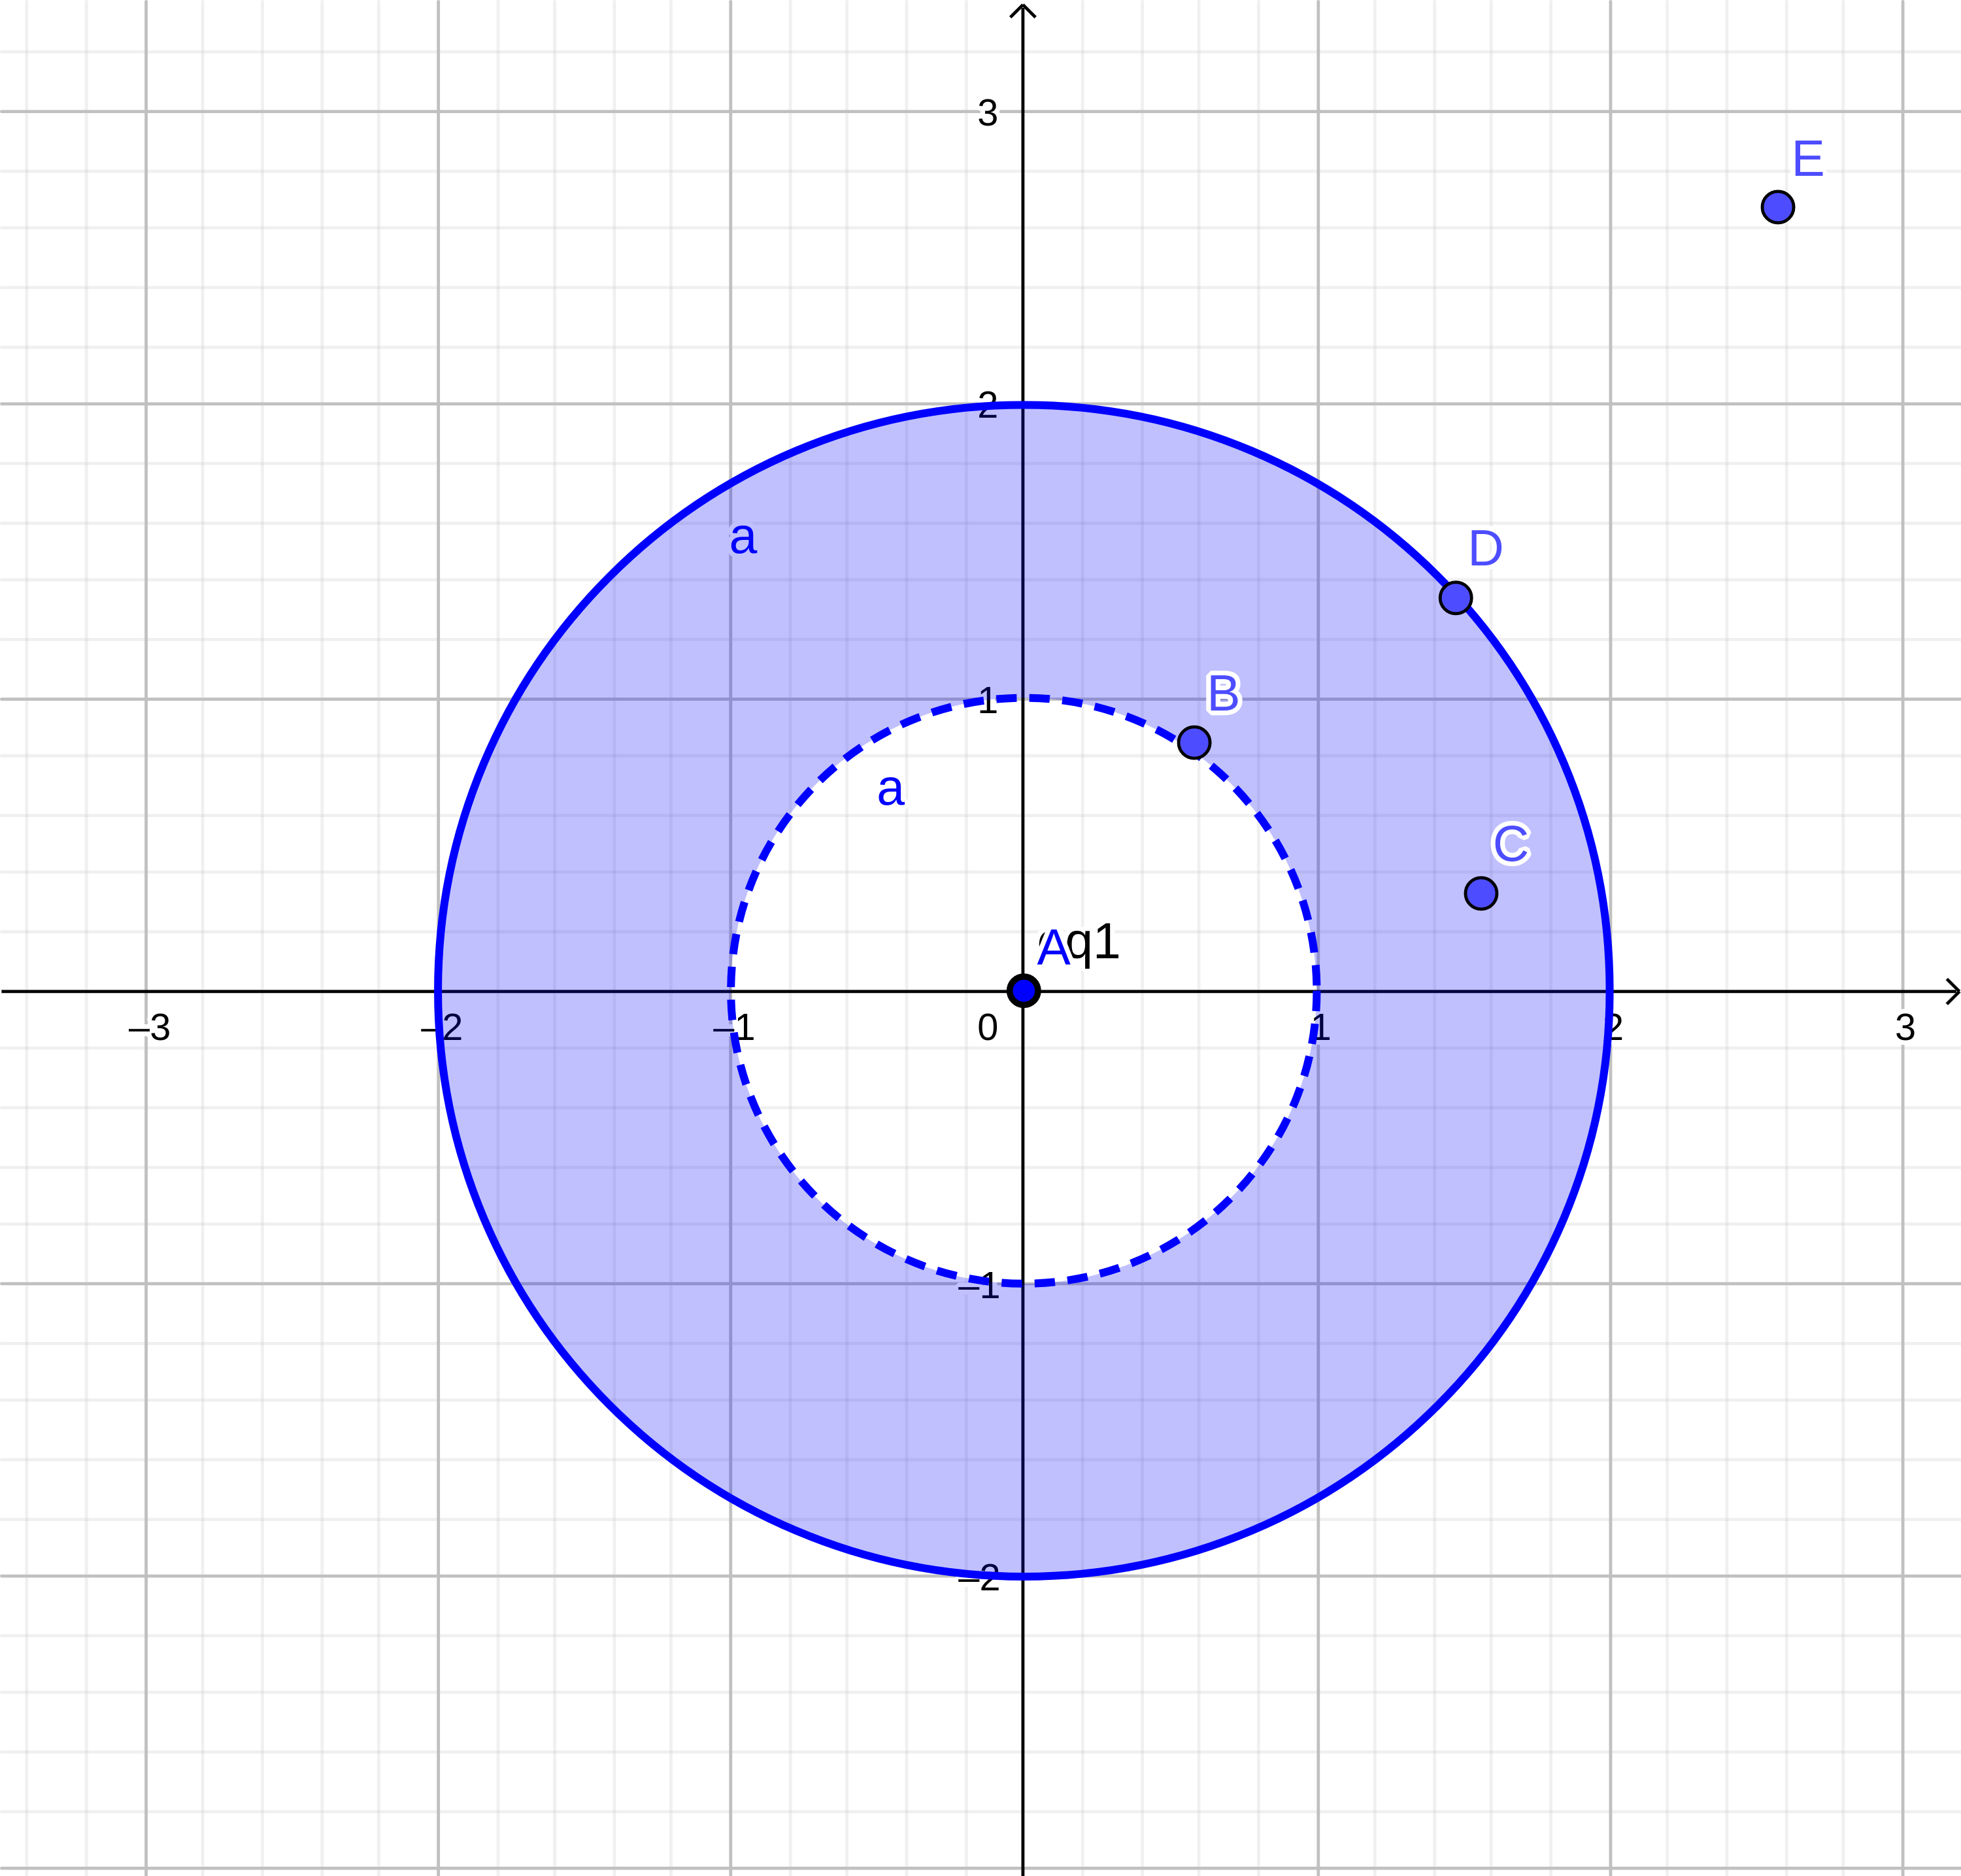
\includegraphics[width=10cm]{./PictureNote/Eg1.png}
              \begin{quote}
              A点是孤立点,因为你可以找到A的一个邻域使得A是该邻域与E的唯一交点,A又是边界点,因为你可以找到A的一个邻域一部分在E中,一部分在E外. 
              
              B点是边界点,因为你可以找到B的一个邻域一部分在E中,一部分在E外.B又是一个聚点,因为B的邻域再小也好都与E有交集。

              C点是内点,也是聚点.

              D点是边界点,是内点,是聚点.

              E点是外点
              \end{quote}
            \end{figure}
        \end{quote}
          
          
    \paragraph{开集}
      若$E$中的每个点都是$E$的内点,则称$E$为开集.(换句话说没有边界)

      例2.$E={(x,y)|1 < x^2+y^2 < 4}$
    \paragraph{连通}
      若对于$E$中的任意两点,都可以用若干条直线段相连接(一条直线段相连称为单连通,多条直线相联通为多连通)且该直线段的点都属于$E$,则称$E$是连通的.(通俗的解释就是$E$是一整块而不是几块加起来的)
    \paragraph{开区域}
      连通的开集
    \paragraph{闭区域}
      开区域加边界
    \paragraph{有界集、无界集}
      可以找到一个点集把该点集包起来,该点集就是有界集,反之则是无界集

    以上所有内容都可推导至n维
    \subsection{二元函数} 
      \paragraph{定义}
        $D$是平面上的一个点集,如果对于每个点$P(x,y) \in D$,变量$z$按照一定的法则总是有唯一确定的值和$P$对应,则$z$是变量$x,y$的二元函数,记为$z=f(x,y)$或$z=f(P)$(简单的说就是两个变量决定一个值,这里定义的是一个标量函数,因为因变元是标量嘛)

        类似的可以定义更多元的函数.
      \paragraph{值域}
        z的所有取值嘛
      \paragraph{定义域}
        一样的解不等式组嘛,求出来应该是一个图形范围.这个点集称为二元函数的平面图形.二元函数的图形实际上通常是一个曲面.
      \subsubsection{多元函数的基本性质}
      \paragraph{奇偶性}
      \paragraph{多元函数的极限}
        设函数$z=f(x,y)$的定义域为D,$P_0(x_0,y_0)$是其聚点,如果
          $$\forall \epsilon > 0 , \exists  \delta > 0 ,0 < |PP_0| = \sqrt{(x-x_0)^2 + (y-y_0)^2} < \delta, \rightarrow |f(x,y) - A| < \epsilon$$
          则$A$为函数$z = f(x,y)$当$x \rightarrow x_0,y \rightarrow y_0$时的极限.
          $$\lim_{(x,y) \to (x_0,y_0)} {f(x,y)} = A$$
          二元函数的极限也叫做二重极限(x和y是同时逼近的).

          二元函数的极限运算法则和一元类似.

          证明极限不存在的方法:

          法1. 找两种特殊的逼近方法使得两个逼近极限不同.
          法2. 令$P(x,y)$沿$y=kx$趋向于$P_0(x_0,y_0)$,若极限值和$k$有关,则可以断言极限不存在.

          一元函数极限的性质,如极限的唯一性、局部有界性、局部保号性

          二次(累次)极限:
            $$\lim_{y \to y_0} {\lim_{x \to x_0} {f(x,y)}}$$
              或
            $$\lim_{x \to x_0} {\lim_{y \to y_0} {f(x,y)}}$$
        性质:
          1. 两个累次极限都存在,不能保证重极限存在,如:
          $$f(x,y) = \frac{xy}{x^2+y^2}$$
          2. 而重极限存在,不能保证累次极限存在,如
          $$f(x,y) = x\sin{\frac{1}{y}} + y\sin{\frac{1}{x}}(xy \neq 0)$$
          3. 若重极限和累次极限都存在,则他们必定相等.
    \paragraph{连续性}
        设n元函数$f(P)$在点集$D$内有定义,$P_0(x_0,y_0)$是D的聚点且点$P_0 \in D$.如果$\lim_{P \to P_0}{f(P)} = f(P_0)$(即$\lim_{P \to P_0} P = P_0,\lim_{P \to P_0}{f(P)} = f(\lim_{P \to P_0} P)$,则称$f(P)$在$P_0$处连续.
      \subparagraph{闭区域上连续函数的性质}
        \begin{quote}
          1. 最大最小值定理:在有界闭区域$D$上的多元连续函数,在$D$上至少取得他的最大值和最小值个一次.

          2. 介值定理:在有界闭区域$D$上的多元连续函数,如果在$D$上取得两个不同的函数值,则它在$D$上取得介于这两值之间的任何值至少一次.

          3. 一致连续性定理*
            $P_1,P_2$接近的时候,$f(P_1)$和$f(P_2)$也很接近.(用$\epsilon,\delta$表达)
        \end{quote}
  \section{偏导数}
        \subsection{定义}
        设函数$z=f(x,y)$在点$(x_0,y_0)$的某一点邻域有定义,当$y$固定在$y_0$而$x$在$x_0$处有增量$\Delta x$时,相应的函数有增量$f(x_0+\Delta x,y_0)-f(x_0,y_0)$,如果$\lim_{\Delta x \to 0}{\frac{f(x_0+\Delta x,y_0)-f(x_0,y_0)}{\Delta x}}$存在,则称此极限为函数$z=f(x,y)$在点$(x_0,y_0)$处对$x$的偏导数,记作:
            $$\frac{\partial z}{\partial x} |_{x=x_0,y=y_0}$$
            或
            $$Z_x|_{x=x_0,y=y_0}$$
            或
            $$f_x(x_0,y_0)$$
        说穿了就是先忽略其他变量(当作常数)只考虑主变量进行求导。
        \subsection{运算法则}
          和一元函数一致(加减乘除,链式法则)
          
          \paragraph{几点说明:}
        \subparagraph{1.}偏导数$\frac{\partial u}{\partial x}$是一个整体记号,不可拆分;
        \subparagraph{2.}求分界点、不连续点处的偏导数要用定义求;
    \subsection{偏导数存在与连续的关系}
        一元函数在某点可导$\Rightarrow$其连续;

        多元函数中在某点偏导数存在$\neq>$其连续;

        例如:
        $$f(x,y)=\begin{cases}
          \frac{xy}{x^2+y^2},x^2+y^2 \neq 0\\
          0,x^2+y^2=0\\
        \end{cases}$$
        多元函数中在某点连续$\neq>$偏导数存在;
        例如:
          $$f(x,y)=\sqrt{x^2+y^2}$$
    \subsection{偏导数的几何意义}
        $f_x(x_0,y_0)$就是曲面被平面$y=y_0$所截得的\emph{曲线}在点$M_0$处的切线对$x$轴的斜率;
    \subsection{高阶偏导数}
        \paragraph{二阶偏导数}
        \subparagraph{纯偏导数}
          对同一个变量二次求导
        \subparagraph{混合偏导数}
          两阶导数分别对不同的变量求导

          二阶混合偏导数什么时候相等?
        \subparagraph{定理:}如果函数$z=f(x,y)$的两个混合偏导数在区域$D$内连续,那么在该区域内这两个二阶混合偏导数相等
  \section{全微分及其概念}
        对于一元函数$y=f(x)$,增量与微分的关系为:
          $$\Delta y = f(x_0+\Delta x) - f(x_0)=A\Delta x + o(\Delta x)$$
          $$A=\frac{dy}{dx}$$
        如此考虑二元函数对$x$和$y$的偏增量:
          $$f(x+\Delta x,y) - f(x,y) = A\Delta x + o(\Delta x)$$
          $$f(x,y+\Delta y) - f(x,y) = B\Delta y + o(\Delta y)$$
        \paragraph{全增量的定义}
          如果函数$z=f(x,y)$在点$(x,y)$的某邻域内有定义,并设$P'(x+\Delta x,y+\Delta y)$为邻域内的任意一点则称这两点的函数值之差为全增量
          $$\Delta z = f(x+\Delta x,y+\Delta y) - f(x,y) $$
          如果$\Delta z$可以表示为:
          $$\Delta z= A\Delta x + B\Delta y + o(\rho)$$
          则称$f(x,y)$在点$(x,y)$处可微分,则函数在该点连续。 
          
          如果$f(x,y)$在区域$D$内都可微,则称该函数在$D$内可微分。
        \subsection{函数可微的条件}
          \paragraph{必要条件}:如果函数$z=f(x,y)$在点$(x,y)$可微分,则该函数的偏导数均存在

          \emph{注意!}如果函数的各个偏导数都存在,函数的全微分并不一定存在!!!
          $$dz = \frac {\partial z}{\partial x} \Delta x + \frac{\partial z}{\partial y} \Delta y $$

          证明:已知$\Delta z = A \Delta x + B \Delta y + o(\rho)$
          
          当$\Delta y = 0$时,$\Delta z = A \Delta x + B \Delta y + o(\rho) = A \Delta x + o(\rho)$
          $$\lim_{\rho \to 0}{o(\rho)}=0$$
          $$\Delta z = A \Delta x$$
          则
          $$\lim_{\Delta x \to 0} {\frac{\partial z}{\partial x}} = A$$
          同理$$\lim_{\Delta y \to 0} {\frac{\partial z}{\partial y}} = B$$
          \paragraph{充分条件}:函数的各个偏导数都存在且\emph{连续},则该函数在点$$(x,y)$$可微分.
  \section{多元复合函数的求导法则}
  \subsection{链式法则}
  前提,几层函数都在点$t$可导。第一层(最表面这一层)可微。则复合函数$f(\varphi(t),\Psi(t)$在$t$点可导,且:
      $$\frac{dz}{dt} = \frac{\partial z}{\partial u}\frac{du}{dt} + \frac{\partial z}{\partial v}\frac{dv}{dt}$$
      \paragraph{推导}
        \begin{quote}
          $dz = \frac{\partial z}{\partial u}du + \frac{\partial z}{\partial v}dv + o(\rho)$

          $\frac{dz}{dt} = \frac{\partial z}{\partial u}\frac{du}{dt} + \frac{\partial z}{\partial v}\frac{dv}{dt} + \frac{o(\rho)}{dt}$

        \end{quote}
      实际上这个定理可以推广到中间变量不是一元函数而是多元函数的情况$z = f[\varphi(x,y),\psi(x,y)]$
      连续求对应元的偏导即可

      可以使用分支路线图进行理解
      \begin{quote}
        特殊的,设$z=f(u,x,y),u=\varphi(x,y)$
        故
          $$
          \frac{\partial z}{\partial x} = \frac{\partial f}{\partial u}\frac{\partial u}{\partial x} + \frac{\partial f}{x}
          $$
      \end{quote}
  
  \subsection{全微分形式不变性}
  函数对中间变量(都是关于底层自变量的函数)和最终自变量的全微分形式一致,因为对于我的$f$来说你的套娃有几层根本无所谓,反正我只看一层。
  \subsection{微分法则}
      和一元一致
  \section{隐函数的求导公式}
  \subsubsection{一个方程的情形}
  1. $F(x,y) = 0$
  \emph{隐函数存在定理1} 设函数$F(x,y)$在点$P(x_0,y_0)$的某一点邻域内具有连续的偏导数\footnote{为了之后可以求隐函数导数},且
  $$F(x_0,y_0) = 0\footnote{保证点满足隐函数关系},F_y(x_0,y_0) \ne 0\footnote{作为分母当然最好不为0}$$
  则方程$F(x,y) = 0$ 且在点$P(x_0,y_0)$的某一邻域内恒能唯一确定一个单值连续的函数$y = f(x)$,他满足条件\emph{$y_0 = f(x_0)$},并有
  $$\frac{dy}{dx} = -\frac{F_x}{F_y}$$
  \paragraph{几何解释}$F(x_0,y_0) = 0$
  见国防科大慕课P34
  \subsubsection{两个及以上方程}
      设函数$u = u(x,y),v = v(x,y)$由方程组
  $$\begin{cases}
    F(x,y,u,v) = 0,\\
    G(x,y,u,v) = 0\\
  \end{cases}$$
  所确定,试推导$\frac{\partial u}{\partial x},\frac{\partial u}{\partial y},\frac{\partial v}{\partial x},\frac{\partial v}{\partial y}$
  
  克莱姆法则来了!
  我们确定一个记号:

  $$J = \frac{\partial (F,G)}{\partial (u,v)} = \begin{vmatrix}
    F_u'&& F_v'\\
    G_u'&& G_v'
  \end{vmatrix}\quad$$
  将方程
  $$\begin{cases}
    F(x,y,u,v) = 0,\\
    G(x,y,u,v) = 0\\
  \end{cases}$$
  两边关于$x$求偏导数得
  $$\begin{cases}
    F_u'\frac{\partial u}{\partial x} + F_v'\frac{\partial v}{\partial x} = -F_x',\\
    G_u'\frac{\partial u}{\partial x} + G_v'\frac{\partial v}{\partial x}= -G_x'\\
  \end{cases}$$
  则我们可以用克莱姆法则了
  \section{微分法在几何上应用}
      \subsection{空间曲线的切线与法平面}
        曲线上有一点$P_0(x_0,y_0,z_0),P(x,y,z)$,对于$P_0P$直线,其方程为:

        $$\frac{x-x_0}{dx} = \frac{y-y_0}{dy} = \frac{z-z_0}{dz}$$
        等式除以$dt$
        $$\frac{x-x_0}{\frac{dx}{dt}} = \frac{y-y_0}{\frac{dy}{dt}} = \frac{z-z_0}{\frac{dz}{dt}}$$
        从上面可以看出空间曲线的切线方程,可以利用曲线的参数方程对参数t求导。
        同时可以用这个方法得到法平面
        参数我们可以选择:
        $$\begin{cases}
          x = x\\
          y = \phi(x)\\
          z = \psi(x)\\
        \end{cases}$$
        此时y,z全部视作关于x的因变量,然后隐函数求导
      \subsection{空间曲面的切平面与法线}
  \section{方向函数与梯度}
      \subsection{方向导数}
      \subsubsection{定义}
      \begin{figure}[htbp]
        \centering
        \caption{方向导数定义}

        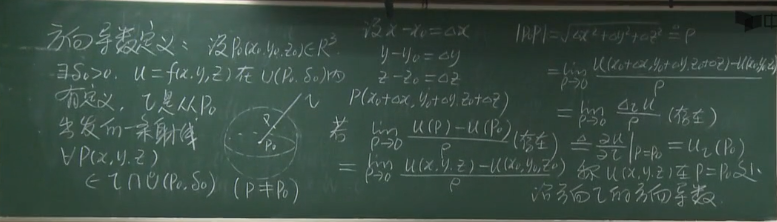
\includegraphics[width = 10cm]{PictureNote/fangxiangdaoshudingyi.png}

      \end{figure}
      注意:仅有三个偏导数都存在未必所有方向导数都存在,我们要加强条件! 
      以$f(x,y)$在$(x_0,y_0)$处为例,若$f_x'(x_0,y_0)$(存在)$= \lim_{\delta x \to 0} {\frac{f(x_0+\delta x,y_0)-f(x_0,y_0)}{\delta x}}$
      \emph{定理(方向导数存在的充分条件)},若$u=u(x,y,z)$在点$P_0(x_0,y_0,z_0)$\textbf{可微},则$u$在点$P_0$点的任意方向$\vec l$的方向导数均存在且
      $$\frac{\partial i}{\partial \vec l}\vert_{p_0} = \frac{\partial u}{\partial x}\vert_{p_0} \cos \alpha + \frac{\partial u}{\partial y}\vert_{p_0} \cos \beta + \frac{\partial u}{\partial z}\vert_{p_0} \cos \gamma$$
      反之不成立!!!!
      证明: 

      $\Delta_{\vec l} u = u(x_0 + \Delta x_0,y_0 + \Delta y_0,z_0 + \Delta z_0) - u(x_0,y_0,z_0) $

      $= \frac{\partial u}{\partial x}\vert_{p_0} \Delta x + \frac{\partial u}{\partial y}\vert_{p_0} \Delta y + \frac{\partial u}{\partial z}\vert_{p_0} \Delta z + o(\rho)$
      易得平行且方向一致的向量的单位向量相同,方向向量为:
      $$\lim_{\rho \to 0} {\frac{\Delta_i u}{\rho}} = \lim_{\rho \to 0}{\frac{\partial u}{\partial x}\vert_{p_0} \frac{\delta x}{\rho} + \frac{\partial u}{\partial y}\vert_{p_0} \frac{\delta y}{\rho} + \frac{\partial u}{\partial z}\vert_{p_0} \frac{\delta z}{\rho} + \frac{o(\rho)}{\rho}}$$
      $$= \frac{\partial u}{\partial x}\vert_{p_0} \cos \alpha + \frac{\partial u}{\partial y}\vert_{p_0} \cos \beta + \frac{\partial u}{\partial z}\vert_{p_0} \cos \gamma$$

      如果求分片函数在孤立点的方向导数一般只能用定义(难以证明可微),初等函数一般用公式

      \subsection{梯度}
  \section{多元函数的极值及其求法及其应用}
  \subsection{多元函数的泰勒公式}
  \textbf{定理}设$z = f(x,y)$在区域$G$上偏导数存在
  
  1. 若$f_x'(x,y) \equiv  0,(x,y)$则$z$仅是$y$的函数

  2. 若$f_y'(x,y) \equiv  0,(x,y)$则$z$仅是$x$的函数

  3. 若$f_x'(x,y) \equiv  0,f_y'(x,y) \equiv  0,(x,y)$则$z$是常函数
  \subsection{二元函数}
      以$z=f(x,y)$为例,设$P_0(x_0,y_0) \in R^2$
      
      极大值和极大值点定义:若$\exists \delta_0 >0$,当$P(x,y)\in U(P_0,\delta_0)$时,都有$f(x,y) \le f(x_0,y_0)$

      称$f(x_0,y_0)$为极大值,$(x_0,y_0)$为极大值点

      极小值和极小值点定义:若$\exists \delta_0 >0$,当$P(x,y)\in U(P_0,\delta_0)$时,都有$f(x,y) \ge f(x_0,y_0)$

      称$f(x_0,y_0)$为极小值,$(x_0,y_0)$为极小值点
      注:极值点一定在区域内部
      一元函数的极值点一定在区间内部的驻点(导数为0或不存在的点),我们能不能把这个结论搬过来呢

      可以!
      
      \subsection{极值点存在的必要条件}
      \paragraph{定理(极值点存在的必要条件)}

        若$z=f(x,y)$在$P_0(x_0,y_0)$处取到极值且$f_x'(x_0,y_0),f_x'(x_0,y_0)$均存在,则$f_x'(x_0,y_0)=0,f_x'(x_0,y_0)=0$,反之不成立

    \subparagraph{证明} 由条件$z=f(x,y)$在点$P_0(x_0,y_0)$处取到极值,不妨设取得极大值,由定义知$\exists \delta_0 >0$,当$P(x,y)\in U(P_0,\delta_0)$时,都有$f(x,y) \le f(x_0,y_0)$

    因此有$f_x(x,y_0) \le f(x_0,y_0),x \in (x_0 - \delta_0,x_0+\delta_0)$,

    知一元函数$f(x,y_0)$在$x=x_0$处取到极大值且$\frac{df(x,y_0)}{dx} \vert_{x=x_0} = f_x'(x_0,y_0)$存在

    由费马定理,则$f_x'(x_0,y_0) = 0 $
    
      同理$f_y'(x_0,y_0) = 0$

      反之不成立,经典例子$f(x,y) = xy$,在$(0,0)$处

      \paragraph{定义:}若$f_x'(x_0,y_0) = 0,f_y'(x_0,y_0)= 0 $称$P_0(x_0,y_0)$为驻点或稳定点

      \textbf{总结}$z = f(x,y)$的极值点一定包含 在区域内部的驻点或者内部偏导数至少有一个不存在的点

      偏导数至少一个不存在的经典例子,$z = \sqrt{x^2+y^2}$在$(x_0,y_0)$处

      \subsection{极值点存在的充分条件}
      \textbf{定理},若$f_x'(x_0,y_0)= 0,f_y'(x_0,y_0) = 0$,设$z=f(x,y)$在$U(P_0,\delta),(\delta > 0)$内具有二阶连续偏导数

      设$f_{xx}'' (x_0,y_0) = A,f_{xy}'' (x_0,y_0) = B,f_{yy}'' (x_0,y_0) = B$
      \paragraph{1.}当$B^2 - AC < 0 $,则$f(x_0,y_0)$确实为极值,此时$A,C$同号,当$ A > 0$,则$f(x_0,y_0)$为极小值
      \paragraph{2.}当$B^2 - AC > 0 $,则$f(x_0,y_0)$不是极值
      \paragraph{3.}当$B^2 - AC = 0 $,则本方法失效

      \subsection{条件极值}
      求 $u = f(x,y,z)=0$在条件$\varphi(x,y,z) = 0$下的极值,称为条件极值

      设在点$P_0(x_0,y_0)$处取得极值
      $\phi (x,y,z) = 0$确定$z = z(x,y)$

  \section{向量和矩阵微分}
\end{document}
